\documentclass[a4paper, 11 pt]{article}


\usepackage{amsfonts}
\usepackage{amsmath}
\usepackage{amsthm}
\usepackage{appendix}
\usepackage{bm}
\usepackage{booktabs}
\usepackage[usenames, dvipsnames]{color} 
\usepackage{graphicx}
\usepackage{epstopdf}
\epstopdfsetup{update}
\usepackage{helvet}
\usepackage{hyperref}
\usepackage{indentfirst}
\usepackage{lscape}
\usepackage{morefloats}
\usepackage{natbib} \bibliographystyle{abbrvnat}\bibpunct{(}{)}{;}{a}{,}{,}
\usepackage{setspace}
\usepackage{subcaption}
\usepackage[capposition=top]{floatrow}
\usepackage{subfloat}
\usepackage[latin1]{inputenc}
\usepackage{tikz}
\usetikzlibrary{trees}
\usetikzlibrary{decorations.markings}


\theoremstyle{plain}
\newtheorem{thm}{Theorem}
\newtheorem{cor}{Corollary}
\newtheorem{lem}[thm]{Lemma}
\newtheorem{proposition}{Proposition}
\newtheorem{assumption}{Assumption}
\newtheorem{definition}{Definition}

%MARGINS
 \topmargin   =  7.0in
 \headheight  =  2.0in
 \headsep     =  0.7in
 \oddsidemargin= 0.0in
 \evensidemargin=0.0in
 \textwidth   =  6.45in
 \headheight  =  0.0in
 \topmargin   =  0.0in
 \textheight  =  9.0in
 \textwidth   =  6.45in
\setlength{\parindent}{4em}
\setlength{\parskip}{1em}

\newcommand{\fmt}{.eps}
%\newcommand{\fmt}{.png}
\hypersetup{                                                                                                    
    colorlinks=true,   
    linkcolor=BlueViolet,
    citecolor=BlueViolet,
    filecolor=BlueViolet,
    urlcolor=BlueViolet
}  




\setcounter{page}{0}
\begin{document}



\title{Fertility Timing and Season of Birth:\\ The Role of Biological and Economic Constraints\thanks{\scriptsize{We thank ... for helpful comments and suggestions. ... Any errors contained in the paper are our own.}}}
\author{Damian Clarke \\ U. of Oxford \and Sonia Oreffice \\ U. of Surrey \& IZA  \and Climent Quintana-Domeque \\ U. of Oxford \& IZA}
\date{April 2015}


%\author{Damian Clarke  \and Sonia Oreffice  \and Climent Quintana-Domeque  }
%\author{Damian Clarke \\ University of Oxford \and Sonia Oreffice \\ University of Surrey and IZA \and Climent Quintana-Domeque \\University of Oxford and IZA}


\maketitle
\thispagestyle{empty}

\begin{abstract}
{....}
\end{abstract}
\emph{JEL Classification Codes}: ....\\
\emph{Keywords}: .....


\newpage
\begin{spacing}{1.4}

%-------------------------------------------------------------------------------
\section{Introduction}
Papers we have mentioned in discussions:
\citet{BucklesHungerman2013,Shigeoka2015,AlbaCaceres2014,Canchoetal2007},
plus I think we mentioned the papers showing short time changes in birth timing
due to tax reforms (such as \citet{GansLeigh2009,LaLumiaetal2015}), etc.

%-------------------------------------------------------------------------------
\section{Data and Descriptive Statistics}
\subsection{USA Birth Data}
\label{bqSscn:USAdata}
Data on all births occurring each year in the United States are collected from 
birth certificate records, and publicly released as the National Vital 
Statistics System (NVSS) by the National Center of Health Statistics. This data 
is available for download for all years (inclusive) between 1968 and 2013, with
all registered births in all states and the District of Columbia reported from 
1984 onwards.\footnote{Prior to 1984, a 50\% sample was released for those 
states which did not submit their birth records on electronic, machine readable 
tape \citep{Martinetal2015}.}  In total, greater than 99\% of births occurring 
in the country are registered \citep{Martinetal2015}. Our main estimation 
sample consists of birth years 2005-2013, and we retain all first births to 
US-born, white, non-hispanic mothers aged between 25 and 45 years at the time
of birth.  This results in 4,863,864 records for live singleton or twin births.  
In many cases we restrict our sample to only single births, in which case the 
estimation sample consists of 4,711,449 first births.

The birth certificate data records a number of important parental and child
covariates and outcomes.  For the mother this includes age, education, smoking
status, and assisted reproductive technology (ART) use. For the newborn, 
measured outcomes include gestation, birthweight, one- and five-minute APGAR, 
and place and time of birth. However, USA birth certificates have gone through 
two important revisions in the variables reported: one in 1989 and the other in 
2003.  These revisions (described fully in \citet{NCHS2000}) were implemented
by states at different points in time.  Prior to 2005 all states had fully 
incorporated the 1989 revision.  In the most recent wave of birth certificate
data (2013), 41 states, containing 90.2\% of all births had switched to the
more recent 2003 revision.  Importantly, the revised data includes a different
measure of education, a wider range of birth outcomes, and does not include
the mother's smoking status. ART use was first released in 2012. These changes
mean that we do not have measures of all covariates for all years.  Complete
details of covariate availability are available in table 
\ref{bqTab:SumStatsNVSS}, and further details regarding birth certificate 
revisions and the effect on reported variables and representativeness of the
country as a whole are provided in appendix \ref{bqScn:datApp}. Finally, from 2005 
onwards public use data does not contain geographic detail released in earlier 
waves of data.  We applied to the National Association for Public Health 
Statistics and Information Systems (NAPHSIS) to receive state identifiers for all 
births for all time periods of our study.\footnote{This data is freely available 
upon application and NAPHSIS review. Full details are provided on the web at
\href{http://www.cdc.gov/nchs/nvss/dvs_data_release.htm}%
{http://www.cdc.gov/nchs/nvss/dvs\_data\_release.htm}.}

Summary statistics are provided in table \ref{bqTab:SumStatsNVSS}.  Of first-%
time mothers in the USA, 84\% are married, and 97\% are aged under 40 years.
The full distribution of mother's age at first birth for 25-45 year-olds is 
presented in figure \ref{bqFig:NVSSages}.  The modal age at first birth of this
sample of women in the USA is 28 years, and the mean age is 30.24 years. A high 
proportion of white mothers from 2005-2013 report having at least some 
post-secondary education (87\%), where this category includes ``some college 
credit, but not a degree'', as well as associate or bachelor degrees and above.  
Of the subset of states and years in which smoking status is reported, 6\% of 
women report smoking at some point during pregnancy.  Of all births, slightly 
more children are born in quarters 2 or 3 (``good season''), at 51\%.  In terms
of birth outcomes, 7\% of babies are classified as low birth weight (LBW) given
that they weigh less than 2,500 grams at birth (the average birth weight is 
slightly more than 3,300g), 10\% are born premature (less than 37 weeks of 
gestation), and 3\% of recorded births are twins.

%-------------------------------------------------------------------------------
\subsection{Spain Birth Data}
We augment results from USA using data on births from Spain. Birth certificate 
records from Spain are released by the National Institute of Statistics (INE) 
with coverage from 1979 to 2013 inclusive. These consist of the universe of 
births registered annually in Spain. Our principal estimation sample consists of 
all first born children who survived one day, born to Spanish mothers. We use 
births from the period 2007 to 2013, given that prior to 2007, education was not 
recorded on birth certificates.  This results in a sample of 1,239,749 live 
births, of which 1,238,685 were singletons.

Like birth certificate data in the USA, Spanish certificates provide mother
and child characteristics, including education and labour market status of the 
mother (and father where present), mother's age at time of birth, marital 
status, and child APGAR, gestation, birthweight, prematurity, and so forth
\citep{INE2013}.  The Spanish records include publicly released data on 
geographical location of birth, at both the provincial and municipal level 
(similar to US states and counties respectively).  Descriptive statistics for
Spanish births are provided in table \ref{bqTab:SumStatsSpain}.  In the same
age group, the average age and proportion of young mothers is similar to data
from USA (32 years and 96\% respectively), however a lower proportion report
being married (64\%), or having at least some post secondary education (53\%).
Spanish newborns are slightly lighter on average than their USA-born 
counterparts (3,200g), however are also less likely to be born prematurely,
or classified as having low birth weight.

%-------------------------------------------------------------------------------
\subsection{Other Variables}
A number of other data sources are consulted, and merged with birth data to
provide time-varying coverage of local conditions at the time of conception.  
This includes Spanish and United States measures of weather and unemployment.  
In each case these are calculated at the year by month by state (or province) 
level, and are merged by conception (not birth) month.  In the case of both USA 
and Spain, we are able to precisely calculate both conception and birth month, 
given that gestation (in weeks) is reported in administrative data.

United States temperature data is provided by the National Centers for 
Environmental Information from 1895 onwards, updated monthly.  We collate 
measures of monthly means, maxima and minima for each state, year and month 
over our time period of analysis as described in \citet{Voseetal2014}. These are 
available for all states with the exception of Hawaii, however are not available 
for the District of Columbia (DC). We assign births that take place in DC 
temperature data from Maryland, a contiguous state.  Spanish climate data at the 
level of the province is calculated from data released by the State Meteorlogical 
Agency (AEMET). This data records the temperature at principal state 
meteorological stations, from which we calculate monthly average, minima and 
maxima. Finally, unemployment data at the level of the state, year and month is 
created from the Bureau of Labor Statistics' (BLS) online monthly time series 
data.\footnote{Full records are available at 
\href{http://download.bls.gov/pub/time.series/la/}%
{http://download.bls.gov/pub/time.series/la/}.} This data comes from the Local 
Area Unemployment Statistics (LAUS) Series, and is avaialable for all states 
plus DC for the entire time period of interest.

\section{Estimation}
\subsection{Season of Birth: Determinants and Effects}

Begin by discussing determinants of season of birth regression for mother $i$ in 
region $j$:
\begin{equation}
\label{eqn:season}
S^{good}_{ij} = \alpha_0 + \alpha_1 young_{ij} + \alpha_2 educ_{ij}  + 
\mathbf{X}_{ij}'\mathbf{\alpha_3} + \mathbf{W}_{j}'\mathbf{\alpha_4} + \mu_j +\nu_{ij}. 
\end{equation}
Here, $S^{good}_{ij}$ refers to a birth in the ``good'' season (quarters 2 and 3),
$\mathbf{X}$ are individual covariates including smoking status and marital status,
and $\mathbf{W}$ are state-specific time-varying indicators such as unemployment
rates and weather in month of conception.  We include state fixed effects $\mu_j$.

Then examine the quality regression for the first-born child of woman $i$:
\begin{equation}
\label{eqn:quality}
Bwt_{ij} = \beta_0 + \beta_1 S^{good}_{ij} + \beta_2 young_{ij} + \beta_3 educ_{ij}  + 
\mathbf{X}_{ij}'\mathbf{\beta_3} + \mathbf{W}_{j}'\mathbf{\beta_4} + \mu_j +\nu_{ij}. 
\end{equation}
We proxy birth quality by birthweight, however also examine other outcomes 
including APGAR, low birth weight indicators, prematurity, and so forth.


%-------------------------------------------------------------------------------
\subsection{A Structural Interpretation of Season of Birth Choices: The Quality%
--Labour Market Tradeoff}
We begin with a young woman $i$ endowed with completed education $Educ_i$.  Each
individual decides sequentially whether or not to have their first birth.  The 
decision is made dynamically, and consists of four periods in which the woman 
can decide to give birth or not: young good season (YG), young bad season (YB), 
old good season (OG) and old bad season (OB). A control variable denoted $b_{it}$ 
describes the optimal entry rule: if $b_{it}=0$, the woman has not yet chosen to 
give birth, and in the period in which she decides to give birth, $b_{it}$ 
switches to 1 forever after. 

\paragraph{Instantaneous Utilities}
In each period the individual faces instantaneous utility of having a birth
($b=1$) or not having a birth ($b=0$) described by:
\begin{eqnarray}
U^{b=1}&=&\ln(w_{it}^{b=1}) + \gamma q_{it} + \varepsilon^{b=1}_{it}, \nonumber \\
U^{b=0}&=&\ln(w_{it}^{b=0}) + \varepsilon^{b=0}_{it}. \nonumber 
\end{eqnarray}
In this framework utility comes from the from market wage or shadow price for 
home labour ($w_{it}$), as well as the biological quality of the child ($q_{it}$)
if a birth has been realised, and a stochastic utility shock only observed once 
arriving to each period ($\varepsilon_{it}$).  For now, it is assumed that these
stochastic shocks are jointly normally distributed each with a mean of zero, 
standard deviation $\sigma_{b=1},\sigma_{b=0}$ and zero covariance.  Each 
$\varepsilon_{it}$ term is assumed to be i.i.d., so past values of each utility
shock have no effect on current realisations.

Wage and birth quality can be thought of as offer functions in each period, and 
are modelled as:
\[
\ln(w_{it})=\alpha_1 Educ_{i} + \alpha_2 Exper_{it} + \alpha_3 Exper_{it}^2
\]
and
\[
q_{it} = \beta_0 + \beta_1 S^{good}_{it} + \beta_2 young_{it} + \beta_3 Educ_{i}.
\]

\paragraph{Bellman Equations} In each of the four periods the state variables
for each individual are (time invariant) education $Educ_i$, accrued labour 
market experience, $Exper_{it}$, and the utility shocks $\varepsilon_{it}$.  
We now denote these state variables as $\Omega_{it}$.  Conditional on state 
variables, we can express the value of remaining childless or deciding to have 
a child in the form of Bellman equations.  The value of remaining childless, 
$V_{it}^{b=0}(\Omega_{it})$, can be expressed as:
\begin{equation}
\label{beEqn:VF0}
V_{it}^{b=0}(\Omega_{it})=U_{it}^{b=0}+\beta E\max
                         [V_{it+1}^{b=0}(\Omega_{it+1}),V_{it+1}^{b=1}(\Omega_{it+1})]
\end{equation}
where $\beta$ is the discount rate.  Similarly, the value of deciding to
give birth is expressed as:
\begin{equation}
\label{beEqn:VF1}
V_{it}^{b=1}(\Omega_{it})=U_{it}^{b=1}+\beta E(V_{t+1}|b_t=1).
\end{equation}
Once the individual decides to give birth, the value function $V_{t+1}|b_t=1$
consists of the discounted expected present value of labour market return and 
child quality, from $t+1$ to the final period.

%-------------------------------------------------------------------------------
\paragraph{Estimating the Model}
The decision of whether or not to have a birth depends upon prior decisions 
regarding births, as well as the prevailing instantaneous utilities.  The
likelihood of observing a first birth in a given period $t$ can then be thought 
of as the intersection of the probability that the individual still remains 
childless at the end of $t-1$, and the probability that the instantaneous 
utility of having a birth is greater than the utility of remaining childless. As 
the error terms $\varepsilon_t^{b=1}$ and $\varepsilon_t^{b=0}$ are assumed to 
be i.i.d., these two events are independent, and the likelihood will be the 
product of these two terms.

Define a vector of parameters $\bm\theta=(\gamma,\beta,\sigma_{b=1},
\sigma_{b=0})$. Then we are interested in writing the likelihood function, which 
for an individual in time $t$ looks like:
\begin{eqnarray}
\mathcal{L}(\bm\theta;b_t=1,U_t^{b=1},U_t^{b=0})&=&
P(b_{t-1}=0|\bm\theta) \times P(U_t^{b=1}-U_t^{b=0}>0|\bm\theta) \nonumber \\
& = & \mathcal{L}(\bm\theta;b_{t-1}=0)\times 
\mathcal{L}(\bm\theta;U_t^{b=1}-U_t^{b=0}>0) \nonumber
\end{eqnarray}
writing this as the log-likelihood gives:
\begin{equation}
\ell(\bm\theta;b_t=1,U_t^{b=1},U_t^{b=0})= \ell(\bm\theta;b_{t-1}=0) 
+ \ell(\bm\theta;U_t^{b=1}-U_t^{b=0}>0)
\end{equation}

We can write the likelihood of the second part of this equation by considering
the probability that $U_t^{b=1}>U_t^{b=0}$:
\begin{eqnarray}
\label{bqEqn:LL2}
Pr(U_t^{b=1}>U_t^{b=0})&=&Pr\{[\ln(w_{it}^{b=1}) + \gamma q_{it} + \varepsilon^{b=1}_{it}]
>[\ln(w_{it}^{b=0}) + \varepsilon^{b=0}_{it}]\} \nonumber \\
&=&Pr[\ln(w_{it}^{b=1})-\ln(w_{it}^{b=0})+ \gamma q_{it} > 
(\varepsilon^{b=1}_{it}-\varepsilon^{b=0}_{it})] 
\end{eqnarray}
given that each of the $\varepsilon$ terms is normally distributed, 
$\varepsilon^{b=1}_{it}-\varepsilon^{b=0}_{it}$ is also normally distributed,
with a mean of zero and a variance of $\sigma_{b=1}^2+\sigma_{b=0}^2$, which for
ease of exposition we will will now denote as $\sigma^2_b$.  We can then simply 
write the likelihood using the well known formula for a normally distributed 
variable as:
\begin{equation}
\ell(\bm\theta;U_t^{b=1}-U_t^{b=0}>0) = \ln\left[\sigma_b^{-1}\cdot\phi
\left(\frac{\ln(w_{it}^{b=1})-\ln(w_{it}^{b=0})+ \gamma q_{it}}{\sigma_b}\right)\right],
\end{equation}
where $\phi(\cdot)$ is the normal $pdf$.

The likelihood of the first part of the equation, $\ell(\bm\theta;b_{t-1}=0)$, can 
be calculated by using the Bellman equations (\ref{beEqn:VF0}) and (\ref{beEqn:VF1}).  
This can be calculated analytically using backwards induction, given that the 
expectation of the value functions is taken over future draws from iid normal 
variables.  \textcolor{blue}{I need to work through the math here, but I think it 
will look somewhat similar to the second part of the log-likelihood discussed above, 
meaning that the log-likelihood can be written as a closed form equation, and can be 
maximised quite easily on the computer.  From this, we estimate $\bm{\theta}$, and 
hence $\gamma$, the parameter which compares the utility from an additional gram of 
birth weight versus the utility from an additional unit of $\ln$(wage).}

Finally then, aggregating over all individuals in each period, we can write the
log-likelihood function to maximise as:
\[
\ell(\bm\theta;b_t=1,U_t^{b=1},U_t^{b=0})= \prod_{i=1}^N\prod_{t=1}^T
\ell(\bm\theta;b_{it-1}=0) + \ell(\bm\theta;U_{it}^{b=1}-U_{it}^{b=0}>0).
\]

\section{Results}
\subsection{Season of Birth Choice: Descriptive Characteristics}

\subsection{Season of Birth Choice: Reduced Form Estimates}

\subsection{Structural Estimates of Birth and Career Timing}




\section{Conclusion}

\newpage
\bibliography{./refs}




\newpage
\section*{Tables}
\input{./../tables/sumStatsnvss.tex}
\input{./../tables/sumsinglenvss.tex}
\input{./../results/nvss/regressions/NVSSBinaryMain.tex}
\begin{landscape}
\input{./../tables/quarterHeterogeneity.tex}
\end{landscape}
\input{./../results/nvss/regressions/NVSSBinaryEdInteract.tex}
\input{./../results/nvss/regressions/NVSSBinaryYoung34.tex}
\input{./../results/nvss/regressions/NVSSseasonMLogit.tex}
\begin{landscape}
\begin{table}[htbp]\centering
\def\sym#1{\ifmmode^{#1}\else\(^{#1}\)\fi}
\caption{Birth Quality by Age and Season (NVSS 2005-2013)}
\scalebox{0.68}{
\begin{tabular}{l*{7}{c}}
\toprule
                    &\multicolumn{1}{c}{(1)}   &\multicolumn{1}{c}{(2)}   &\multicolumn{1}{c}{(3)}   &\multicolumn{1}{c}{(4)}   &\multicolumn{1}{c}{(5)}   &\multicolumn{1}{c}{(6)}   &\multicolumn{1}{c}{(7)}   \\
                    &       APGAR   & Birthweight   &   Gestation   &         LBW   &   Premature   &        Twin   &        VLBW   \\
\midrule
Aged 25-39          &       0.043***&     130.718***&       0.598***&      -0.055***&      -0.064***&      -0.054***&      -0.010***\\
                    &     [0.004]   &     [2.581]   &     [0.011]   &     [0.001]   &     [0.001]   &     [0.001]   &     [0.000]   \\
Bad Season          &       0.002   &      -5.653   &      -0.011   &       0.004** &       0.002   &       0.001   &      -0.001*  \\
                    &     [0.005]   &     [3.585]   &     [0.015]   &     [0.002]   &     [0.002]   &     [0.001]   &     [0.001]   \\
Young$\times$ Bad S &      -0.005   &      -4.781   &      -0.014   &      -0.001   &       0.001   &       0.001   &       0.002***\\
                    &     [0.005]   &     [3.638]   &     [0.015]   &     [0.002]   &     [0.002]   &     [0.001]   &     [0.001]   \\
College Educ        &       0.045***&      77.112***&       0.181***&      -0.025***&      -0.021***&       0.010***&      -0.006***\\
                    &     [0.001]   &     [0.917]   &     [0.004]   &     [0.000]   &     [0.000]   &     [0.000]   &     [0.000]   \\
&&&&&&&\\
Constant            &       8.756***&    3121.397***&      38.034***&       0.150***&       0.194***&       1.075***&       0.028***\\
                    &     [0.004]   &     [2.775]   &     [0.012]   &     [0.001]   &     [0.001]   &     [0.001]   &     [0.001]   \\
\midrule
R-squared           &        0.00   &        0.00   &        0.00   &        0.00   &        0.00   &        0.00   &        0.00   \\
Observations        &     3551931   &     3603294   &     3610749   &     3613920   &     3613920   &     3613920   &     3613920   \\
\bottomrule
\multicolumn{8}{p{15cm}}{\begin{footnotesize}Sample consists of all
first born children of US-born, white, non-hispanic mothers
\end{footnotesize}}\end{tabular}}\end{table}

\end{landscape}
\begin{landscape}
\input{./../tables/qualityHeterogeneity.tex}
\end{landscape}
\begin{landscape}
\input{./../results/nvss/regressions/QualityAllComb.tex}
\end{landscape}
\input{./../tables/sumStatsSpain.tex}
\input{./../tables/sumSpain.tex}
\begin{landscape}
\input{./../results/spain/regressions/spainBinary.tex}
\end{landscape}
\begin{landscape}
\input{./../results/spain/regressions/spainQualityEduc.tex}
\end{landscape}
\begin{landscape}
\input{./../results/spain/regressions/spainQualityGestFix.tex}
\end{landscape}


\newpage
\section*{Figures}
\begin{figure}[htpb!]
  \begin{center}
  \caption{Mother's Age at First Birth}
  \label{bqFig:NVSSages}
  \includegraphics[scale=0.82]{./../results/nvss/graphs/ageDescriptive.eps} 
  \end{center}
\end{figure}

\vspace{8mm}


\begin{figure}[htpb!]
  \begin{center}
  \caption{Difference in Births: \% Good Season--\% Bad Season (Education)}
  \label{bqFig:diffQ}
  \includegraphics[scale=0.82]{../results/nvss/graphs/birthQdiff.eps}
  \end{center}
  {\footnotesize Note to figure \ref{bqFig:diffQ}: `Young' refers to 25-39 years
  old at first birth.  `Old' refers to 40-45 at first birth.}
\end{figure}


\begin{figure}[htpb!]
  \begin{center}
  \caption{Difference in Births (\% Good Season - \% Bad Season)}
  \label{fig:NVSSbirthsAges}
  \includegraphics[scale=0.8]{./../results/nvss/graphs/birthQdiff_4Ages.eps}
  \end{center}
\end{figure}

\begin{figure}[htpb!]
\begin{center}
\caption{Births per Month (25-39): Northern and Southern Hemisphere Countries}
\label{bqFig:excess}
\includegraphics[scale=1.15]{../results/countries/combinedMonthExcess.eps}
\end{center}
{\footnotesize Note to figure \ref{bqFig:excess}: Each panel is one country.  Bars
represent the difference between expected (evenly spaced) births and actual births.  
Births for USA are 2005-2013, for Chile 2000-2012, for Mexico 2000-2005 and for Spain 
2013.  Earlier births are used for Mexico as reporting can occurr after the date of
the event while for each of the other country data is recorded at the time of birth.  
Average temperatures per month for each country are plotted in appendix figure 
\ref{bqFig:excessTemp}.}
\end{figure}
\vspace{5mm}

\begin{figure}[htpb!]
  \begin{center}
  \centering
  \caption{Proportion of Mothers Reporting any ART}
  \label{bqfig:NVSSART}
  \includegraphics[scale=0.82]{./../results/nvss/graphs/ART.eps}
  \end{center}
  {\footnotesize Note to figure \ref{bqfig:NVSSART}: Questions on ART use are 
  only included in 2012-2013 birth certificate data.}
\end{figure}

\clearpage

\begin{figure}[htpb!]
  \begin{center}
  \centering
  \caption{Proportion of Twins Born by Age}
  \label{fig:NVSSTwins}
  \includegraphics[scale=0.77]{./../results/nvss/graphs/twinPrevalence.eps}
  \end{center}
\end{figure}


\begin{figure}[htpb!]
\caption{Conception and Births: 25-39 Year-olds}
\hspace{8.0cm}\textbf{Realized Season} \vspace{4mm}\\
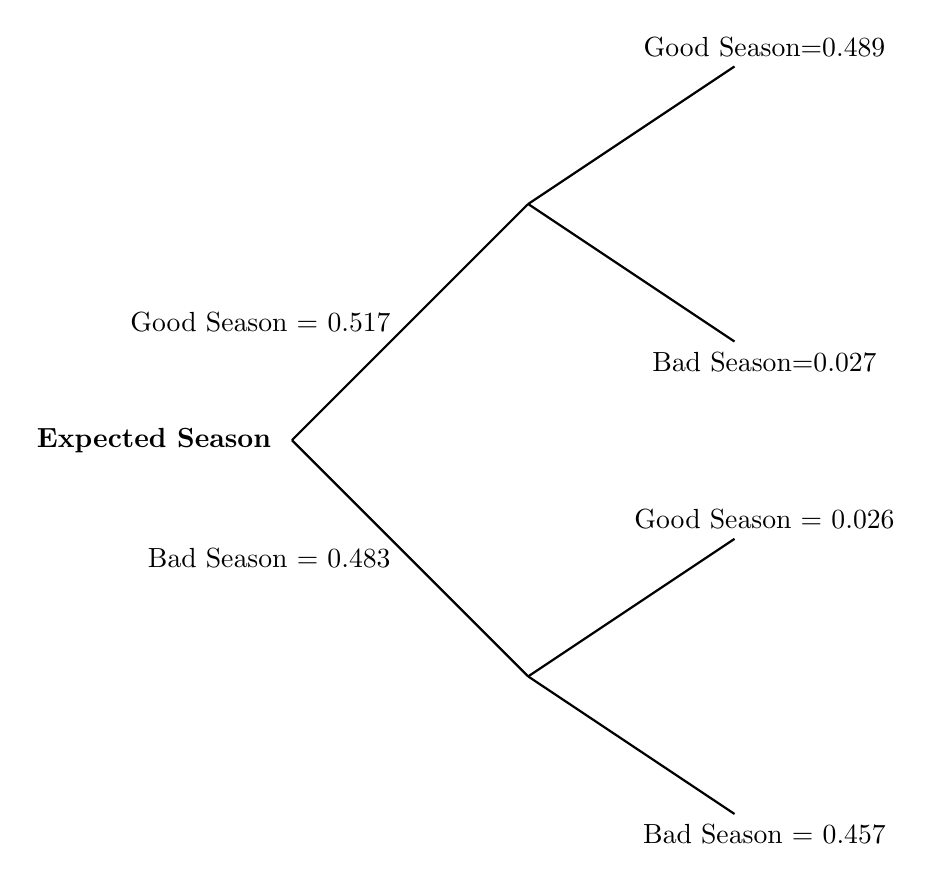
\begin{tikzpicture}[thick,
    level/.style={level distance=3cm},
    level 2/.style={sibling distance=6cm},
    level 3/.style={sibling distance=4cm}
]
\coordinate
child[grow=right, level distance=0pt] {
        child  {
            child {
                node {Bad Season = 0.457}
                edge from parent 
            }
            child {
                node {Good Season = 0.026}
                edge from parent
            }
            edge from parent
            node [left] {Bad Season = 0.483 \ }
        }
        child {
            child {
                node {Bad Season=0.027}
                edge from parent
            }
            child {
                node {Good Season=0.489}
                edge from parent  
            }
            edge from parent 
            node [left] {Good Season = 0.517 \ }
        }
        node [left] {\textbf{Expected Season\ \ }}
    };
\end{tikzpicture}
\end{figure}


\begin{figure}[htpb!]
\caption{Conception and Births: 40-45 Year-olds}
\hspace{8.0cm}\textbf{Realized Season} \vspace{4mm}\\
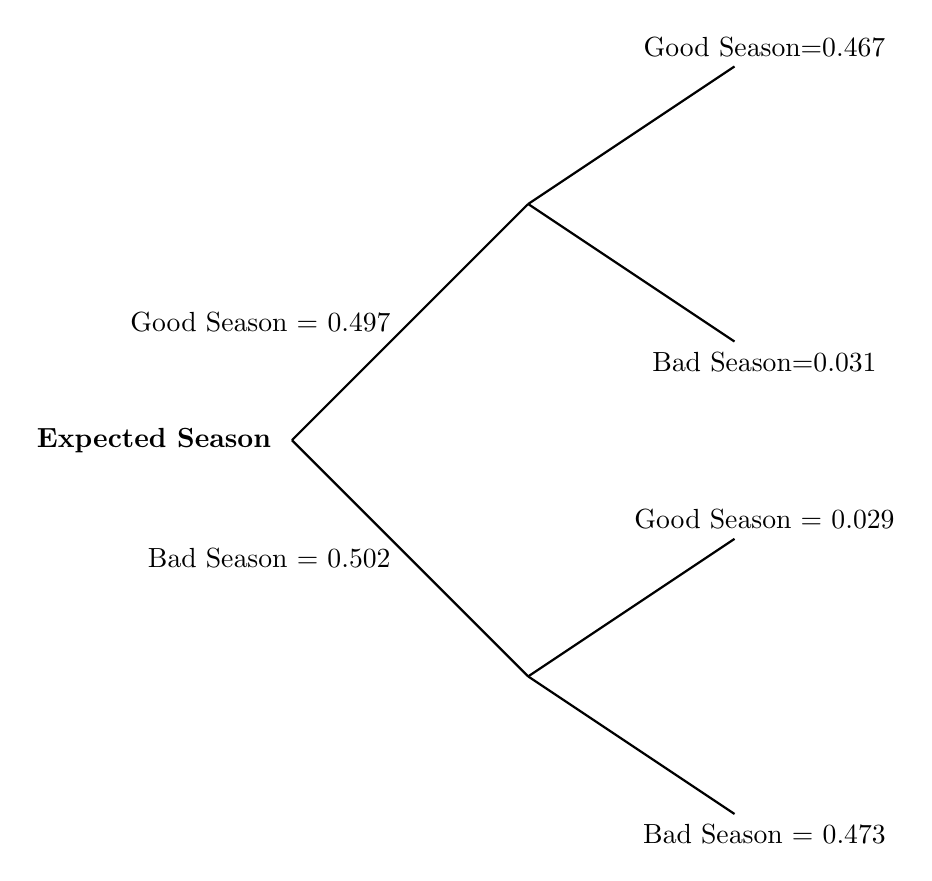
\begin{tikzpicture}[thick,
    level/.style={level distance=3cm},
    level 2/.style={sibling distance=6cm},
    level 3/.style={sibling distance=4cm}
]
\coordinate
child[grow=right, level distance=0pt] {
        child  {
            child {
                node {Bad Season = 0.473}
                edge from parent 
            }
            child {
                node {Good Season = 0.029}
                edge from parent
            }
            edge from parent
            node [left] {Bad Season = 0.502 \ }
        }
        child {
            child {
                node {Bad Season=0.031}
                edge from parent
            }
            child {
                node {Good Season=0.467}
                edge from parent  
            }
            edge from parent 
            node [left] {Good Season = 0.497 \ }
        }
        node [left] {\textbf{Expected Season\ \ }}
    };
\end{tikzpicture}
\end{figure}


\begin{figure}[htpb!]
\begin{center}
  \centering
  \caption{Good Season by State (Young)}
  \includegraphics[scale=0.34]{./../results/nvss/graphs/maps/young.png}
  \label{fig:mapYoung}
\end{center}
\end{figure}

\begin{figure}[htpb!]
\begin{center}
  \centering
  \caption{Good Season by State (Old)}
  \includegraphics[scale=0.34]{./../results/nvss/graphs/maps/old.png}
  \label{fig:mapOld}
\end{center}
\end{figure}

\begin{figure}[htpb!]
\begin{center}
  \centering
  \caption{Temperature and good Quarter: Young (Spain)}
  \includegraphics[scale=0.8]{./../results/spain/graphs/youngTempCold.eps}
  \label{fig:mapYoung}
\end{center}
\end{figure}
\clearpage

\begin{figure}[htpb!]
\begin{center}
  \centering
  \caption{Temperature and good Quarter: Old (Spain)}
  \includegraphics[scale=0.8]{./../results/spain/graphs/oldTempCold.eps}
  \label{fig:mapOld}
\end{center}
\end{figure}

\begin{figure}[htpb!]
\centering
\caption{Child quality: Birthweight (grams)}
\label{QBwt}
\includegraphics[scale=0.8]{../results/nvss/graphs/AllQuality_birthweight_.eps}
\end{figure}
\vspace{1cm}

\begin{figure}[htpb!]
\centering
\caption{Child quality: Birthweight (grams)}
\label{QApgar}
\includegraphics[scale=0.8]{../results/nvss/graphs/Quality_birthweight_.eps}
\end{figure}
\vspace{1cm}





\clearpage
\appendix
\section{Appendix Tables}
\input{./../results/nvss/regressions/NVSSBinaryFDeaths.tex}
\begin{table}[htbp]\centering
\def\sym#1{\ifmmode^{#1}\else\(^{#1}\)\fi}
\caption{Birth Quarter and Age (NVSS 2005-2013)}
\scalebox{0.8}{
\begin{tabular}{l*{4}{c}}
\toprule
                    &\multicolumn{1}{c}{(1)}   &\multicolumn{1}{c}{(2)}   &\multicolumn{1}{c}{(3)}   &\multicolumn{1}{c}{(4)}   \\
                    & Good Season   & Good Season   & Good Season   & Good Season   \\
\midrule
Aged 25-39          &       0.019***&       0.019***&       0.020***&       0.006   \\
                    &     [0.001]   &     [0.001]   &     [0.002]   &     [0.005]   \\
College Educ        &               &               &       0.010***&      -0.005   \\
                    &               &               &     [0.001]   &     [0.005]   \\
College$\times$ Aged 25-39&               &               &               &       0.015***\\
                    &               &               &               &     [0.005]   \\
Constant            &       0.497***&       0.497***&       0.488***&       0.501***\\
                    &     [0.001]   &     [0.001]   &     [0.002]   &     [0.005]   \\
\midrule
R-squared           &        0.00   &        0.00   &        0.00   &        0.00   \\
Observations        &     4871628   &     4871628   &     3613920   &     3613920   \\
Year FE&&Y&Y&Y\\ \bottomrule
\multicolumn{5}{p{12cm}}{\begin{footnotesize}Sample consists of all
first born children of US-born, white, non-hispanic mothers
\end{footnotesize}}\end{tabular}}\end{table}

\begin{landscape}
\input{./../results/bord2/regressions/NVSSQualityEducAll.tex}
\end{landscape}
\begin{landscape}
\begin{table}[htbp]\centering
\def\sym#1{\ifmmode^{#1}\else\(^{#1}\)\fi}
\caption{Birth Quarter and Age (NVSS 2005-2013)}
\scalebox{0.8}{
\begin{tabular}{l*{4}{c}}
\toprule
                    &\multicolumn{1}{c}{(1)}   &\multicolumn{1}{c}{(2)}   &\multicolumn{1}{c}{(3)}   &\multicolumn{1}{c}{(4)}   \\
                    & Good Season   & Good Season   & Good Season   & Good Season   \\
\midrule
Aged 25-39          &       0.019***&       0.019***&       0.020***&       0.006   \\
                    &     [0.001]   &     [0.001]   &     [0.002]   &     [0.005]   \\
College Educ        &               &               &       0.010***&      -0.005   \\
                    &               &               &     [0.001]   &     [0.005]   \\
College$\times$ Aged 25-39&               &               &               &       0.015***\\
                    &               &               &               &     [0.005]   \\
Constant            &       0.497***&       0.497***&       0.488***&       0.501***\\
                    &     [0.001]   &     [0.001]   &     [0.002]   &     [0.005]   \\
\midrule
R-squared           &        0.00   &        0.00   &        0.00   &        0.00   \\
Observations        &     4871628   &     4871628   &     3613920   &     3613920   \\
Year FE&&Y&Y&Y\\ \bottomrule
\multicolumn{5}{p{12cm}}{\begin{footnotesize}Sample consists of all
first born children of US-born, white, non-hispanic mothers
\end{footnotesize}}\end{tabular}}\end{table}

\end{landscape}
\begin{landscape}
\begin{table}[htbp]\centering
\def\sym#1{\ifmmode^{#1}\else\(^{#1}\)\fi}
\caption{Birth Quarter and Age (NVSS 2005-2013)}
\scalebox{0.8}{
\begin{tabular}{l*{4}{c}}
\toprule
                    &\multicolumn{1}{c}{(1)}   &\multicolumn{1}{c}{(2)}   &\multicolumn{1}{c}{(3)}   &\multicolumn{1}{c}{(4)}   \\
                    & Good Season   & Good Season   & Good Season   & Good Season   \\
\midrule
Aged 25-39          &       0.019***&       0.019***&       0.020***&       0.006   \\
                    &     [0.001]   &     [0.001]   &     [0.002]   &     [0.005]   \\
College Educ        &               &               &       0.010***&      -0.005   \\
                    &               &               &     [0.001]   &     [0.005]   \\
College$\times$ Aged 25-39&               &               &               &       0.015***\\
                    &               &               &               &     [0.005]   \\
Constant            &       0.497***&       0.497***&       0.488***&       0.501***\\
                    &     [0.001]   &     [0.001]   &     [0.002]   &     [0.005]   \\
\midrule
R-squared           &        0.00   &        0.00   &        0.00   &        0.00   \\
Observations        &     4871628   &     4871628   &     3613920   &     3613920   \\
Year FE&&Y&Y&Y\\ \bottomrule
\multicolumn{5}{p{12cm}}{\begin{footnotesize}Sample consists of all
first born children of US-born, white, non-hispanic mothers
\end{footnotesize}}\end{tabular}}\end{table}

\end{landscape}
\input{./../results/1970s/regressions/NVSSseasonMLogit.tex}
\input{./../results/1990s/regressions/NVSSseasonMLogit.tex}
\begin{landscape}
\input{./../results/1970s/regressions/QualityAllCombnoFE.tex}
\end{landscape}
\begin{landscape}
\input{./../results/1990s/regressions/QualityAllCombnoFE.tex}
\end{landscape}


\clearpage
\appendix
\section{Appendix Figures}
%\begin{figure}[htpb!] 
%\begin{center}
%  \centering  
%  \caption{Education and Conception Month}
%  \includegraphics[scale=0.7]{./../results/nvss/graphs/conceptionMonthDropout.eps}  
%  \label{fig:concepEduc} 
%\end{center}
%\floatfoot{\textsc{Notes to figure \ref{fig:concepEduc}}: Graph plots the proportion
%of conceptions by month for 25-39 year old women by education level.  Refer to figure
%\ref{bqFig:concepMonth} for additional notes.}
%\end{figure} 

\begin{figure}[htpb!]
\centering
\caption{Younger versus older women births (Spain)}
\label{bqFig:YoungvOldSpain}
  \centering
  \includegraphics[scale=0.82]{../results/spain/graphs/youngMonths.eps}
\floatfoot{\textsc{Notes to figure}: Each point and standard error comes from a regression
of birth month $x$ on a binary indicator of being young (25-39).
}
\end{figure}


\begin{figure}[htpb!]
\begin{center}
\caption{Temperature and Good Quarter (Spain)}
\label{fig:tempSpain}
\begin{subfigure}{.5\textwidth}
  \centering
  \includegraphics[scale=0.55]{./../results/spain/graphs/youngTempCold.eps}
  \caption{Young Mothers}
  \label{fig:tempSpainYoung}
\end{subfigure}%
\begin{subfigure}{.5\textwidth}
  \centering
  \includegraphics[scale=0.55]{./../results/spain/graphs/oldTempCold.eps}
  \caption{Old Mothers}
  \label{fig:tempSpainOld}
\end{subfigure}
\end{center}
\floatfoot{\textsc{Notes to figure}: See notes to figure 
\ref{fig:tempUSAYoung}. Monthly temperature data is 
collected from the Spanish State Meteorology Agency (AEMET).}
\end{figure}



\section{Data Appendix}
\label{bqScn:datApp}
\subsection{NVSS Birth Certificate Data}
A brief description of USA birth certificate data is provided in section 
\ref{bqSscn:USAdata} of the paper.  As discussed, the format of US birth
certificates has undergone two important revisions: the first in 1989
and the second in 2003.  The date of adoption of these revisions varies 
by state.  By 2013 41 states or territories had adopted the revised (2003)
format, while the reaminder still follow the 1989 format.\footnote{The full
birth certificate for each revision is reproduced as figures 1 and 2 in
\citet{MenackerMartin2005}.  Over time the adoption of the 2003 certificate 
was as follows: 2005: 12 (31\%), 2006: 19 (49\%), 2007: 22 (53\%), 2008: 27 
(65\%), 2009: 28 (66\%), 2010: 33 (76\%), 2011: 36 (83\%), 2012: 38 (86\%),
and 2013: 41 (90\%).  In each case the first number refers to the number
of states, while the parenthesis indicates the percent of births in revised
states.}

In all cases where variable coding differs between the revised and unrevised
certificates (principally education for mother and father), we use the revised
2003 coding of the variables.  The reason we do this is because after 2008,
variables which are exclusive to 1989 certificates are no longer reported.
Figure \ref{bqFig:educMissing} illustrates this pattern.  The dotted line 
represents the proportion of observations for maternal education which are
reported in the 1989 format, while the bars represent the proportion 
\emph{missing} in the 2003 format.  From 2005-2008, all missing 2003 revision
variables are recorded in the 1989 format.  However, from 2009 onwards only
the 2003 revision of education is reported, meaning that those states who
still use the 1989 standard certificate do not have publicly released education
data.  As expected, these are not missing at random, given that educational
attainment varies considerably by state (see table \ref{bqTab:missingEduc}).
In each case when these variables are used, we include full year and state
fixed effects.  
\begin{figure}[htpb!]
\caption{Missing Education Data by Time}
\label{bqFig:educMissing}
\includegraphics[scale=0.74]{../results/nvss/graphs/missingEduc.eps}
\end{figure}
\input{./../results/nvss/regressions/NVSSMissingScale.tex}


\end{spacing}
\end{document}







\begin{eqnarray}
\label{struc1}
\max_{\{s,a\}} u(w,b) &\text{s.t.}& w=f(age,educ,\mathbf{X},\varepsilon_w) \\ 
\label{struc2}
&& b=\mu(age,s,\mathbf{X},\varepsilon_b)                                  \\ 
\label{struc3}
&& s=\phi(age,educ,\varepsilon_s). 
\end{eqnarray}

Here $u(\cdot), f(\cdot), \mu(\cdot)$ and $\phi(\cdot)$ are functions and 
$\mathbf{\varepsilon}=(\varepsilon_w,\varepsilon_s,\varepsilon_b)$ are 
unobserved shocks.  To close the structural model we must attach functional
form to the four functions, and make distributional assumptions for $\varepsilon$.

Functional form for equations (\ref{struc2}) and (\ref{struc3}) can be quite simple, 
as it is precisely what we are estimating in equations (\ref{eqn:season}) and 
(\ref{eqn:quality}) respectively.  From our results we know very clearly that:
\[
\frac{\partial b}{\partial s^{good}}>0 \text{\ and \ }
\frac{\partial s^{good}}{\partial age}<0.
\]
It is also generally the case that:
\[
\frac{\partial w}{\partial age}>0.
\]
The wage equation in (\ref{struc1}) could be Mincerian, depending on $age$ and 
$age^2$, as well as education, and is calculated at the level of the state, 
(perhaps using data from CPS or similar to get wage).  Finally, we define $u(w,b)$ 
as a Cobb-Douglas
or CES function (or some other logical form), and assume that $\varepsilon$ is
drawn from a trivariate normal.  We can thus write down a log-likelihood function,
and use our birth data to maximise this function, estimating the parameters in
$f(\cdot), \mu(\cdot)$ and $\phi(\cdot)$, which allows us to quantify the
trade-off between ``having a child today'' versus ``having a child tomorrow'' 
with the relative (market and shadow) prices of labor, as measured by wages, and 
child quality, proxied by birthweights.
